\begin{lstlisting}
56789
\end{lstlisting}
\begin{exercise}
\begin{figure}[H]
\centering
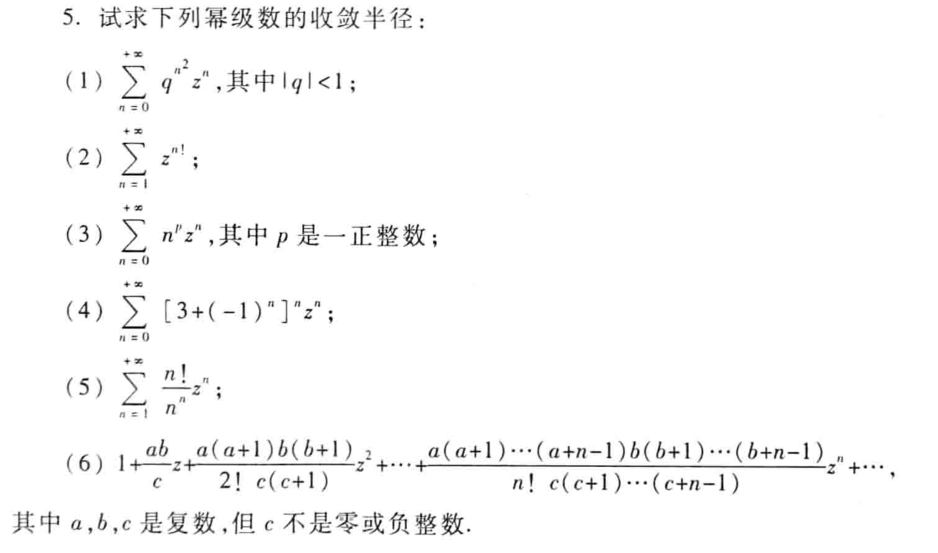
\includegraphics[width=\textwidth]{3-hw7-2025041510.png}
% \caption{}
\label{}
\end{figure}
\end{exercise}
(1) $\limsup_{ n \to \infty } \sqrt[n]{ q^{n^2} }=\limsup_{ n \to \infty }q^{n}=0$ then $R=\infty$.

(2) $\sum_{n=1}^{\infty}z^{n!}=\sum_{n=1}^{\infty}a_nz^{n}$, where
\[
a_n=\begin{cases}
1 & \text{if }n=k!\text{ for some }k \\
0 & \text{otherwise}
\end{cases}
\]
Then $\limsup_{ n \to \infty }\sqrt[n]{ a_n }=1$, $R=\frac{1}{\limsup_{ n \to \infty }\sqrt[n]{ a_n }}=1$.

(3) $\limsup_{ n \to \infty }\sqrt[n]{ n^{p} }=\limsup_{ n \to \infty }\exp\left( \frac{p\ln n}{n} \right)=1$ then $R=\frac{1}{\limsup_{ n \to \infty }\sqrt[n]{ n^{p} }}=1$.

(4) $\limsup_{ n \to \infty }\sqrt[n]{ [3+(-1)^{n}]^{n} }=4$ then $R=\frac{1}{4}$.

(5) $\limsup_{ n \to \infty }\sqrt[n]{ \frac{n!}{n^{n}} }=\limsup_{ n \to \infty }\sqrt[n]{ \frac{1}{n^{n}}\cdot\sqrt{ 2\pi n }\left( \frac{n}{e} \right)^{n}(1+o(1)) }=e^{-1}$. Then $R=e$.

(6)
\[
a_n=\frac{\Gamma(a+n)\Gamma(b+n)\Gamma(c)}{\Gamma(a)\Gamma(b)\Gamma(c+n)\cdot n!}
\]
\begin{lemma}
\[
\Gamma(\alpha+1)=\alpha^\alpha e^{-\alpha} \sqrt{2 \pi \alpha}\left(1+\frac{1}{12 \alpha}+O\left(\alpha^{-2}\right)\right), \lvert \alpha \rvert  \rightarrow+\infty
\]
\end{lemma}
\[
\begin{aligned}
\limsup_{ n \to \infty } \sqrt[n]{ \lvert a_n \rvert  } & =
\limsup_{ n \to \infty } \sqrt[n]{ \left\lvert  \frac{\Gamma(a+n)\Gamma(b+n)\Gamma(c)}{\Gamma(a)\Gamma(b)\Gamma(c+n)\cdot n!}  \right\rvert  } \\
 & =
\limsup_{ n \to \infty } \sqrt[n]{ \left\lvert  \frac{(a+n-1)^{a+n-1}(b+n-1)^{b+n-1}e^{ -(a+b+2n-2) }2\pi\sqrt{ (a+n-1)(b+n-1) }\Gamma(c) }{\Gamma(a)\Gamma(b)(c+n-1)^{c+n-1}e^{ -(c+n-1) }\sqrt{ 2\pi(c+n-1) }\sqrt{ 2\pi n }n^{n}e^{ -n }}  \right\rvert  } \\
 & =\limsup_{ n \to \infty } \sqrt[n]{ \frac{n^{a+n-1}\cdot n^{b+n-1}e^{ -(a+b-2)}e^{ -2n }2\pi \cdot n\cdot\Gamma(c) }{\Gamma(a)\Gamma(b)n^{c+n-1}n\cdot2\pi \cdot n^{n}\cdot e^{ -n }e^{ -c+1-n }} } \\
 & =\limsup_{ n \to \infty } \sqrt[n]{ \frac{\Gamma(c)}{\Gamma(a)\Gamma(b)}e^{ c-a-b+1 }n^{a+b-c-1} } \\
 & =1
\end{aligned}
\]
Thus $R=1$.

\begin{exercise}
\begin{figure}[H]
\centering
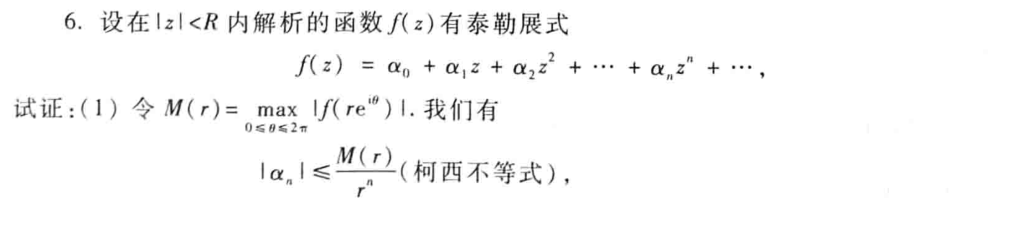
\includegraphics[width=\textwidth]{4-hw7-2025041510.png}
% \caption{}
\label{}
\end{figure}
\begin{figure}[H]
\centering
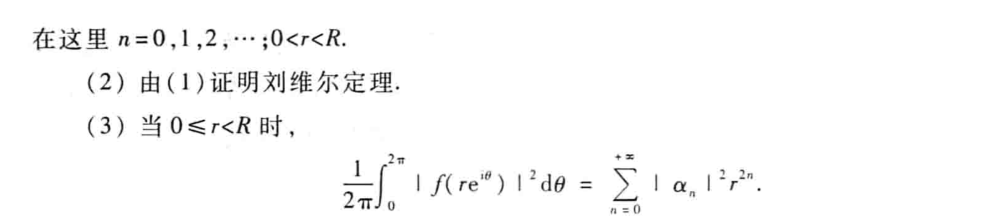
\includegraphics[width=\textwidth]{5-hw7-2025041510.png}
% \caption{}
\label{}
\end{figure}
\end{exercise}
\begin{proof}
(1)
\[
\alpha _n=\frac{1}{2\pi i}\oint_{\lvert z \rvert =r} \frac{f(z)}{z^{n+1}} \, \mathrm{d}z
\]
Then
\[
\lvert \alpha _n \rvert \leq \frac{1}{2\pi }\oint_{\lvert z \rvert =r} \frac{\lvert f(z) \rvert }{\lvert z \rvert ^{n+1}} \, \mathrm{d}z  \leq \frac{1}{2\pi}2\pi r\frac{M(r)}{r^{n+1}}=\frac{M(r)}{r^{n}}
\]
(2)
If $f$ is entire, since $M(r)$ is bounded, then for each $n\geq1$, let $r\to \infty$,
\[
\lvert \alpha _n \rvert \leq \frac{M(r)}{r^{n}}\to0
\]
Therefore $f\equiv a_0$ is constant.

(3)
\[
\begin{aligned}
\frac{1}{2\pi}\int_{0}^{2\pi} \lvert f(re^{ i\theta }) \rvert ^2 \, \mathrm{d}\theta  & =\frac{1}{2\pi}\int_{0}^{2\pi} f(re^{ i\theta })\overline{f(re^{ i\theta })} \, \mathrm{d}\theta  \\
 & =\frac{1}{2\pi }\int_{0}^{2\pi} \sum_{n=0}^{\infty} \alpha _nr^{n}e^{ in\theta }\sum_{m=0}^{\infty}\overline{\alpha _m}r^{m}e^{ -im\theta }  \, \mathrm{d}\theta \\
  & =\frac{1}{2\pi}\sum_{n=0}^{\infty} \sum_{m=0}^{\infty} \int_{0}^{2\pi} \alpha _n \overline{\alpha _m}r^{n+m}e^{ i\theta(n-m) }  \, \mathrm{d}\theta \\
  & =\frac{1}{2\pi}\sum_{n=0}^{\infty} \sum_{m=0}^{\infty} \int_{0}^{2\pi} \alpha _n \overline{\alpha _m}r^{n+m}e^{ i\theta(n-m) }\delta _{mn}  \, \mathrm{d}\theta \\
 & =\frac{1}{2\pi}\sum_{n=0}^{\infty}\int_{0}^{2\pi} \alpha _n \overline{\alpha _n}r^{2n}  \, \mathrm{d}\theta \\
 & =\sum_{n=0}^{\infty} \lvert \alpha _n \rvert ^2 r^{2n}         
\end{aligned}
\]
\end{proof}

\begin{exercise}
\begin{figure}[H]
\centering
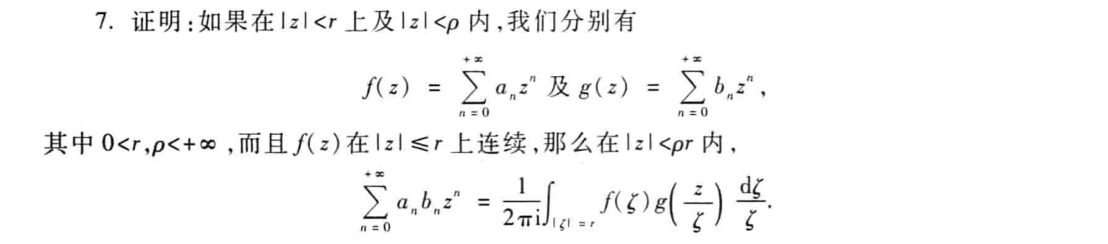
\includegraphics[width=\textwidth]{6-hw7-2025041510.png}
% \caption{}
\label{}
\end{figure}
\end{exercise}
\begin{proof}
\[
\begin{aligned}
 & \frac{1}{2\pi i }\oint_{\lvert \zeta \rvert =r} \sum_{n=0}^{\infty} a_n\zeta^{n}\sum_{m=0}^{\infty} b_m\frac{z^{m}}{\zeta^{m}}\frac{1}{\zeta}  \, \mathrm{d}\zeta   \\
= & \sum_{m=0}^{\infty} z^{m}\left( \sum_{n=0}^{\infty} \frac{1}{2\pi i} \oint_{\lvert \zeta \rvert =r} \frac{a_nb_m}{\zeta^{m-n+1}} \, \mathrm{d}\zeta  \right) \\
= & \sum_{m=0}^{\infty} z^{m}\left( \sum_{n=0}^{\infty} \frac{1}{2\pi i} \oint_{\lvert \zeta \rvert =r} \frac{a_nb_m}{\zeta^{m-n+1}} \delta_{mn}\, \mathrm{d}\zeta  \right) \\
= & \sum_{m=0}^{\infty} a_mb_mz^{m}
\end{aligned}
\]
\end{proof}

\begin{exercise}
\begin{figure}[H]
\centering

\includegraphics[width=\textwidth]{7-hw7-2025041510.png}
% \caption{}
\label{}
\end{figure}
\end{exercise}
\begin{proof}
\[
\lvert e^{ z }-1 \rvert =\left\lvert  \sum_{n=1}^{\infty} \frac{z^{n}}{n!}  \right\rvert \leq \sum_{n=1}^{\infty} \frac{\lvert z \rvert ^{n}}{n!}=e^{ \lvert z \rvert  }-1
\]
Let $f(x)=xe^{ x }-e^{ x }+1$, $x\in \mathbb{R}^{+}$, then
\[
f'(x)=xe^{ x }\geq 0
\]
$f(x)\geq f(0)=0$. Thus
\[
f(\lvert z \rvert )\geq 0\implies \lvert z \rvert e^{ \lvert z \rvert  }\geq e^{ \lvert z \rvert  }-1
\]
\end{proof}

\begin{exercise}
\begin{figure}[H]
\centering
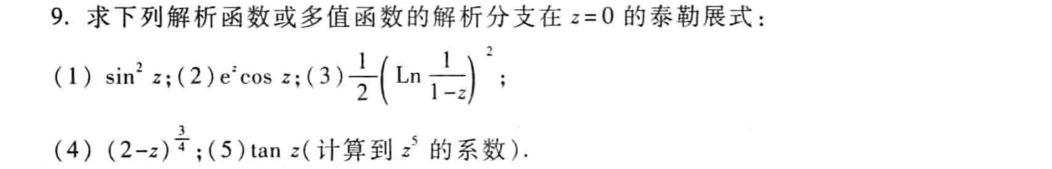
\includegraphics[width=\textwidth]{8-hw7-2025041510.png}
% \caption{}
\label{}
\end{figure}
\end{exercise}
(1)
\[
\sin ^2z=\frac{1}{2}(1-\cos2z)=\frac{1}{2}\left( 1-\sum_{n=0}^{\infty} \frac{(-1)^{n}z^{2n}}{(2n)!} \right)=\sum_{n=1}^{\infty} \frac{(-1)^{n+1}z^{2n}}{2\cdot(2n)!}
\]
(2)
\[
\begin{aligned}
e^{ z }\cos z & =\mathrm{Re}(e^{ z }\cdot e^{ iz })=\mathrm{Re}(e^{ (1+i)z })=\mathrm{Re}\left( \sum_{n=0}^{\infty} \frac{(1+i)^{n}z^{n}}{n!} \right) \\
 & =\mathrm{Re}\left( \sum_{n=0}^{\infty} \frac{2^{\frac{n}{2}}e^{ i\pi \frac{n}{4} }z^{n}}{n!}  \right) \\
 & =\sum_{n=0}^{\infty} \frac{2^{\frac{n}{2}}\cos\left( \frac{n\pi}{4} \right)z^{n}}{n!}
\end{aligned}
\]
(3)
\[
\begin{aligned}
\frac{1}{2}\left( \mathrm{Ln}\frac{1}{1-z} \right)^{2} & =\frac{1}{2}(2k\pi-\ln(1-z))^2=\frac{1}{2}\left( 2k\pi+\sum_{n=1}^{\infty} \frac{z^{n}}{n} \right)^2 \\
 & =\frac{1}{2}\left( 4k^2\pi^{2}+4k\pi \sum_{n=1}^{\infty} \frac{z^{n}}{n}+\sum_{n=2}^{\infty} \left( \frac{2}{m} \sum_{m=1}^{n-1} \frac{1}{m} \right)z^{n} \right) \\
 & =2k^2\pi^{2}+2k\pi \sum_{n=1}^{\infty} \frac{z^{n}}{n}+\sum_{n=2}^{\infty} \left( \frac{1}{n} \sum_{m=1}^{n-1} \frac{1}{m} \right)z^{n}
\end{aligned} 
\]
(4) 主值支:
\[
(2-z)^{\frac{3}{4}}=2^{\frac{3}{4}}\left( 1-\frac{z}{2} \right)^{\frac{3}{4}}=2^{\frac{3}{4}}\cdot \sum_{n=0}^{\infty} \left( -\frac{z}{2} \right)^{n}\cdot\frac{\Gamma\left( \frac{3}{4}+n \right)}{\Gamma\left( \frac{3}{4} \right)}=\sum_{n=0}^{\infty} \frac{(-1)^{n}\Gamma\left( \frac{3}{4}+n \right)}{\Gamma\left( \frac{3}{4} \right)2^{n-\frac{3}{4}}}z^{n}
\]
(5)
\[
\tan z=\frac{\sin z}{\cos z}=z+\frac{1}{3} z^3+\frac{2}{15} z^5+\cdots \quad\left(|z|<\frac{\pi}{2}\right)
\]